\subsection{Esercizio 15}
Usare la \textit{function} del precedente esercizio per risolvere, a partire dal vettore iniziale
nullo, i seguenti sistemi nonlineari, utilizzando tolleranze $tol = 1e-3$, $1e-8$, $1e-13$:
\begin{eqnarray*}
    f_1(x) = \left(\begin{array}{c}
        (x^{2}_{1} + 1)(x_2 - 2) \\
        exp(x_1 - 1) + exp(x_2 - 2) - 2
    \end{array}\right), & & f_2(x) = \left(\begin{array}{c}
        x_1 - x_2x_3                   \\
        exp(x_1 + x_2 + x_3 - 3) - x_2 \\
        x_1 + x_2 + 2x_3 - 4
    \end{array}\right).
\end{eqnarray*}
Tabulare i risultati ottenuti, commentandone l'accuratezza.
\newline \textbf{Soluzione:}
% Eseguendo il codice \nameref{cod:15} si ottengono i seguenti risultati:

% \begin{figure}[h]
%     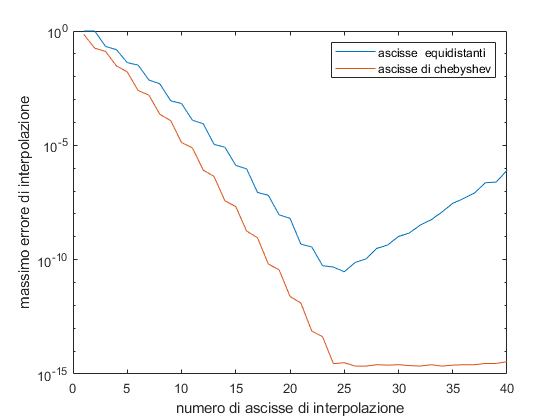
\includegraphics[scale=0.8]{capitolo4/interpol.png}
%     \caption{risultati interpolazione}
%     \label{fig:15}
% \end{figure}


% Per le ascisse di chebyshev, si ha una decrescita esponenziale dell'errore massimo per $ n \le 25$ per poi assestarsi a circa $2\cdot10^{-15}$ per n successivi.
% Per quanto riguarda le ascisse equidistanti invece, si può notare come l'errore massimo torni  a crescere esponenzialmente per $n >25$. I risultati confermano
% il mal condizionamento del problema di interpolazione polinomiale quando vengono usate ascisse d'interpolazione equidistanti,